\input ../preamble

\begin{document}

{\Huge

  \centerline{\bf TTIC 31230, Fundamentals of Deep Learning}
  \bigskip
  \centerline{David McAllester, April 2017}
  \vfill
  \centerline{\bf Generative Adversarial Networks (GANs)}
  \vfill
\vfill
\vfill

\slide{Modeling Distributions (Cross Entropy)}

{\color{red}
\begin{eqnarray*}
  \Phi^* & = & \argmin_\Phi E_{y \sim \mathrm{Pop}} \;- \log Q_\Phi(y) \\
  \\
  \\
  \\
  \Phi^* & = & \argmin_\Phi E_{(x,y) \sim \mathrm{Pop}} \;- \log Q_\Phi(y|x)
\end{eqnarray*}
}

\anaslide{Variational AutoEncoders}

\bigskip

$$Q_\Psi(\hat{z}|y) \hspace{4ex}  Q_\Phi(\hat{z}) \hspace{7ex} \;\hat{y}_\Phi(\hat{z})$$

\bigskip
\centerline{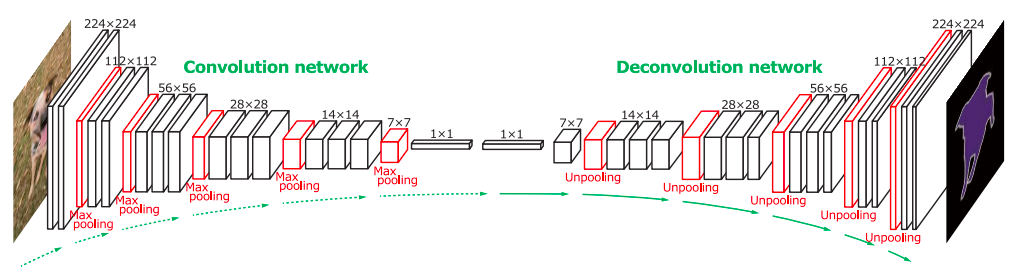
\includegraphics[width=6in]{../images/Deconv}}
\centerline{\large [Hyeonwoo Noh et al.]}
\bigskip
\begin{eqnarray*}
  \Phi^* & = & \argmax_\Phi E_{y \sim \mathrm{Pop}} \;\log Q_\Phi(y) \;\; \mbox{(Cross Entropy)}\\
  \\
  \log Q_\Phi(y) & \geq & \expectsub{\hat{z} \sim {\color{red} P_\Psi(\hat{z}|y)}}{\ln Q_\Phi(\hat{z},y)} + H({\color{red} P_\Psi(\hat{z}|y)})
  \;\;\;\mbox{(ELBO)}
\end{eqnarray*}

\anaslideplain{Generative Adversarial Networks (GANs)}

\bigskip
$$\epsilon \sim \mathrm{noise} \hspace{22ex} \;\hat{y}_\Phi(\epsilon)$$

\bigskip
\centerline{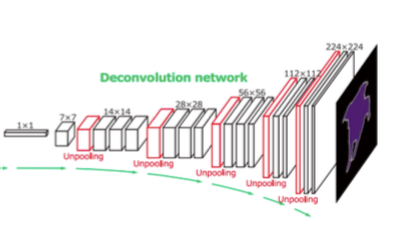
\includegraphics[width=4in]{../images/halfdeconv}}
\centerline{\large [Hyeonwoo Noh et al.]}

\bigskip
In a GAN a distribution is modeled by a {\bf generator} --- there is no encoder.

\slide{GANs, Goodfellow et al., 2014 (also Schmidhuber 1992)}

Cross entropy loss on $Q_\Phi$ is replaced by

$${\color{red} \Phi^* = \argmax_\Phi \; \min_\Psi \;\expectsub{(y,s) \sim (\mathrm{Pop}\; \uplus \;Q_\Phi)}{-\log Q_\Psi(s|y)}}$$

\vfill
$\Phi$ is the generator.

\vfill
$y$ is either drawn from $Q_\Phi$ or from $\pop$ (with equal probabiity) and $s$ is a flag telling which.

\vfill
$\Psi$ is the discriminator --- the descriminator must predict $s$ from $y$.

\slide{The Theorem}

$${\color{red} \Phi^* = \argmax_\Phi \; \min_\Psi \;\expectsub{(y,s) \sim (\mathrm{Pop}\; \uplus \;Q_\Phi)}{-\log Q_\Psi(s|y)}}$$

\vfill
{\bf Theorem:} If $Q_\Phi(y)$ and $Q_\Psi(s|y)$ are universally expressive (can represent any distribution) then
$Q_{\Phi^*} = \mathrm{Pop}.$

\slide{Generated Bedrooms(DC GANS, Radford et al., ICLR 2016)}

\centerline{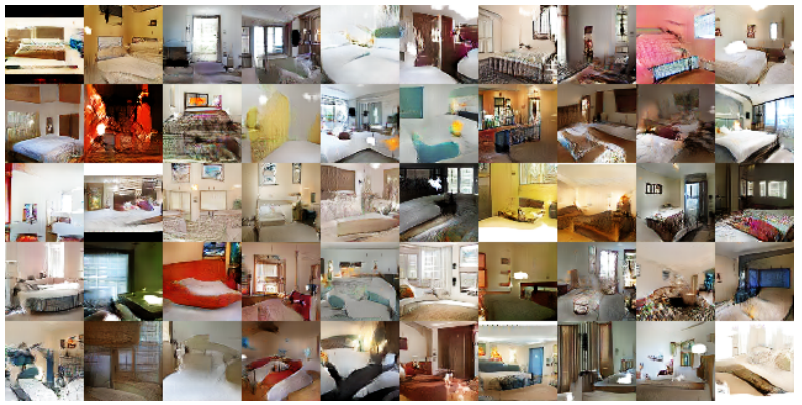
\includegraphics[width = 10in]{../images/Bedrooms}}

\slide{Interpolated Faces}

[Ayan Chakrabarti]

\centerline{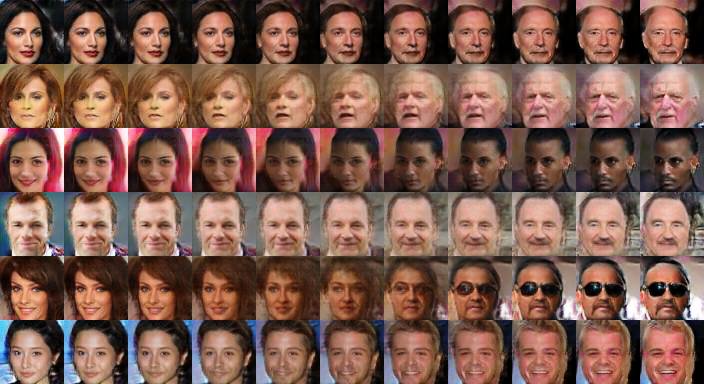
\includegraphics[width = 9in]{../images/interp}}

\slideplain{Image Arithmetic (DC GANS, Radford et al., ICLR 2016)}

\centerline{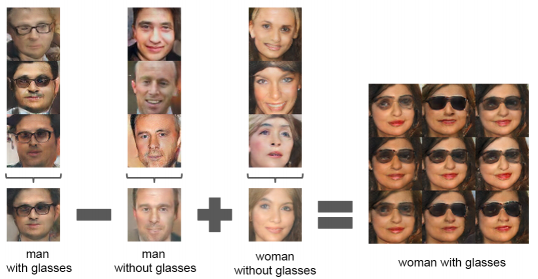
\includegraphics[width = 9in]{../images/ImageFeatures}}

\slide{GANs on Imagenet}

\centerline{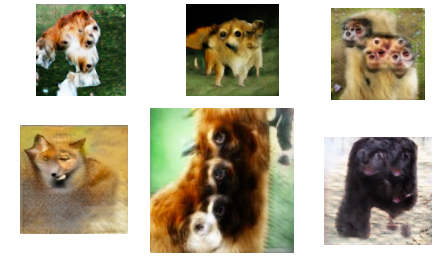
\includegraphics[width = 9in]{../images/BadGAN}}


\slide{Conditional GANs}

All distribution modeling methods apply to conditional distributions.

$${\color{red} \Phi^* = \argmax_\Phi \; \min_\Psi \;\expectsub{(x,y,s) \sim (\mathrm{Pop}\; \uplus \;\mathrm{Pop}(x)Q_\Phi(y|x))}
  {-\log Q_\Psi(s|x,y)}}$$

\slide{Image-to-Image Translation (Isola et al., 2016)}

\centerline{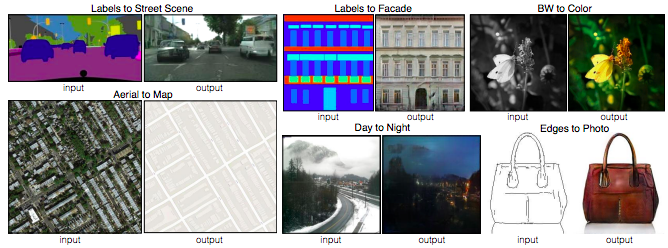
\includegraphics[width = 8.0in]{../images/cGAN0}}

\slide{U-Nets (Ronnenberger et al. 2015)}

\centerline{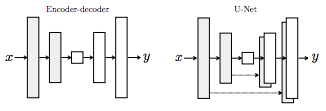
\includegraphics[width = 8.0in]{../images/Unet}}

\slide{Image-to-Image Translation (Isola et al., 2016)}

\centerline{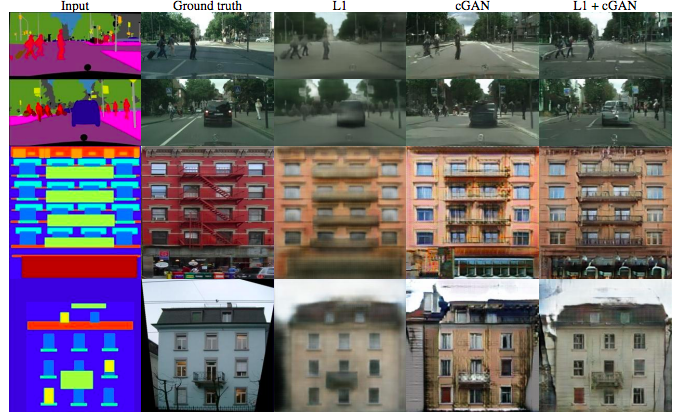
\includegraphics[width = 8.0in]{../images/cGAN1}}

\slide{Arial Photo to Map and Back}

\centerline{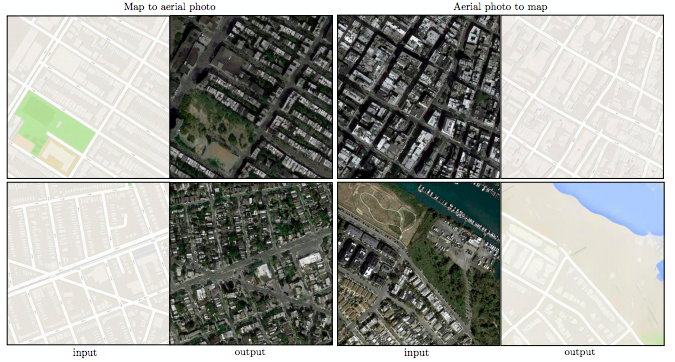
\includegraphics[width = 8.0in]{../images/cGAN2}}

\slide{Colorization}

\centerline{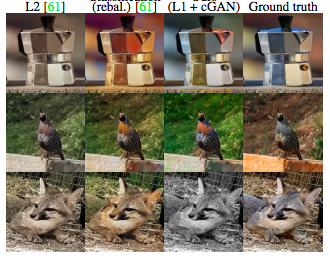
\includegraphics[width = 6.0in]{../images/cGAN3}}

\slide{Semantic Segmentation}

\centerline{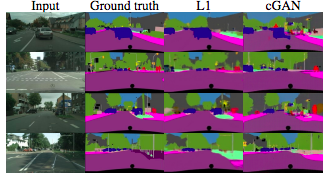
\includegraphics[width = 8.0in]{../images/cGAN4}}

\slide{Cycle Gans (Zhu et al., 2017)}

\centerline{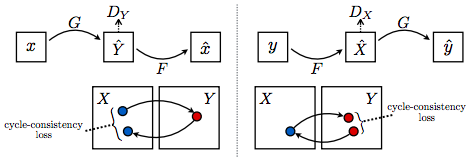
\includegraphics[width = 8.0in]{../images/Cycle2}}


\slide{Cycle Gans}

\centerline{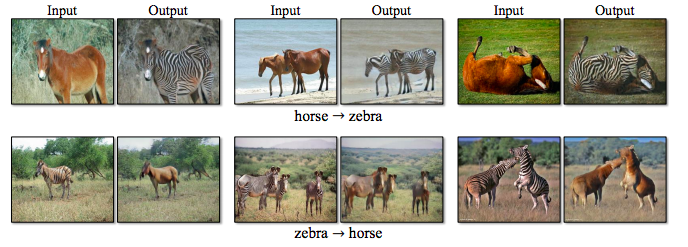
\includegraphics[width = 11.0in]{../images/Cycle3}}

\slide{Cycle Gans}

\centerline{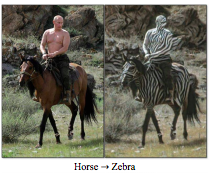
\includegraphics[width = 6.0in]{../images/Cycle4}}

\slidetwo{Cycle Training of Machine Translation}
         {Lample et al, 2017, also Artetxe et al., 2017}

\centerline{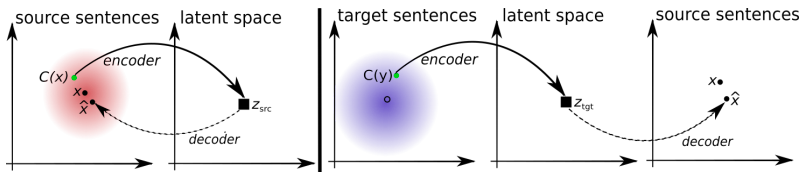
\includegraphics[width = 10.0in]{../images/Cycle5}}

\slide{Text to Speech (Saito et al. 2017)}

\centerline{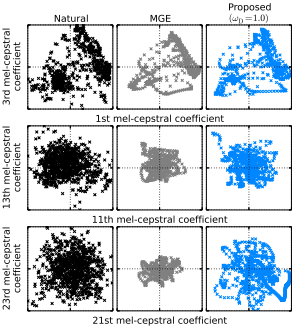
\includegraphics[width = 3.0in]{../images/Txt2spchGAN}}

\vfill
Minimum Generation Error (MGE) uses {\color{red} perceptual distortion} ---
a distance between the feature vector of the generated sound wave and the
feature vector of the original.

\vfill
{\color{red}Perceptual Naturalness} can be enforced by a discriminator.

\slideplain{Adversarial Domain Adaptation (Tzeng et al. 2017)}

\centerline{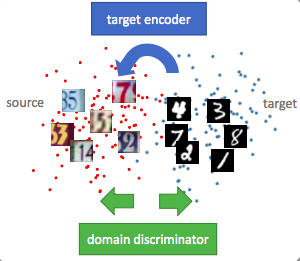
\includegraphics[width = 5.0in]{../images/AdvDomainAdapt}}

\slide{Issues}

\centerline{Jensen-Shannon Divergence}

\vfill
\centerline{Vanishing Gradients}

\vfill
\centerline{Unstable Training}

\vfill
\centerline{Mode Collapse}

\vfill
\centerline{Measuring Perfomance}

\slide{Jensen-Shannon Divergence}

$${\color{red} \Phi^* = \argmax_\Phi \; \min_\Psi \;\expectsub{(y,s) \sim (\mathrm{Pop}\; \uplus \;Q_\Phi)}{- \log Q_\Psi(s|y)}}$$

\vfill
\begin{eqnarray*}
\Psi^*(\Phi) & = & \argmin_\Psi \; \expectsub{(y,s) \sim (\mathrm{Pop}\; \uplus \;Q_\Phi)}{- \log Q_\Psi(s|y)}
\end{eqnarray*}

\vfill
$$Q_{\Psi^*(\Phi)}(s=1|y) = \frac{P(y,s=1)}{P(y)} = \frac{\mathrm{Pop}(y)}{\mathrm{Pop}(y) + Q_\Phi(y)}$$

\eject

\begin{eqnarray*}
\Phi^*  & = & \argmax_\Phi \; \expectsub{(y,s) \sim (\mathrm{Pop}\; \uplus \;Q_\Phi)}{- \log Q_{\Psi^*(\Phi)}(s|y)} \\
\\
  \\
  & = & \argmax_\Phi\; \frac{1}{2}  \expectsub{(y,1) \sim \mathrm{Pop}}{- \log \frac{\mathrm{Pop}(y)}{\mathrm{Pop}(y) + \pi(y|\Phi)}} \\
  & & \;\;\;\;\;\;\; + \frac{1}{2}  \expectsub{(y,-1) \sim Q_\Phi}{- \log \frac{Q_\Phi(y)}{\mathrm{Pop}(y) + Q_\Phi(y)}} \\
  \\
  \\
  & = & \argmax_\Phi \;1 -\frac{1}{2} KL(\mathrm{Pop},A) - \frac{1}{2} KL(Q_\Phi,A)
\end{eqnarray*}

$$A(y)  =  \frac{1}{2}(\mathrm{Pop}(y) + Q_\Phi(y))$$

\slide{Jensen-Shannon Divergence (JSD)}

We have arrived at the Jensen-Shannon divergence.

$${\color{red} \Phi^* = \argmin_\Phi \;\;\mathrm{JSD}(\mathrm{Pop},Q_\Phi)}$$

\vfill
$${\color{red} \mathrm{JSD}(P,Q) = \frac{1}{2} KL\left(P,\frac{P + Q}{2}\right) + \frac{1}{2} KL\left(Q, \frac{P + Q}{2}\right)}$$

\vfill
$$0 \leq \mathrm{JSD}(P,Q) = \mathrm{JSD}(Q,P) \leq 1\ \;\mbox{(in bits)}$$

\slide{Vanishing Gradients}

The discriminator typically ``wins''.

\vfill
The log loss goes to zero (becomes exponentially small) and there is no gradient to guide the generator.

\vfill
In this case the learning stops and the generator is blocked from minimizing $\mathrm{JSD}(\mathrm{Pop},Q_\Phi)$.

\slide{A Heuristic Fix}

We continue to use

$$\Psi^*(\Phi) = \argmin_\Psi \;\expectsub{(y,s) \sim (\mathrm{Pop}\; \uplus \;Q_\Phi)}{- \log Q_\Psi(s|y)}$$

\vfill
But switch the optimization for $\Phi$ from
$$\Phi^* = \argmax_\Phi E_{y \sim Q_\Phi}\; - \log Q_\Psi(-1|y)$$

to
$$\Phi^* = \argmin_\Phi E_{y \sim Q_\Phi}\;- \log Q_\Psi(1|y)$$

\vfill
It can be shown that $- \log Q_\Psi(1|y)$ is essentially the margin of the binary classifier $\Psi$.

\slide{Converting to Cross Entropy (Goodfellow)}

$$\Psi^*(\Phi) = \argmin_\Psi \;\expectsub{(y,s) \sim (\mathrm{Pop}\; \uplus \;Q_\Phi)}{- \log Q_\Psi(s|y)}$$

\vfill
$$\mbox{Assume:}\;\;\; Q_{\Psi^*}(1|y) = \frac{\mathrm{Pop}(y)}{\mathrm{Pop}(y) + Q_\Phi(y)}$$

\vfill
\begin{eqnarray*}
  \mbox{Define:}\;\;\; f_{\Psi^*}(y) & \doteq & \frac{Q_{\Psi^*}(1|y)}{Q_{\Psi^*}(-1|y)} \\
\\
& = & \frac{\mathrm{Pop}(y)}{Q_\Phi(y)}
\end{eqnarray*}

\slide{Converting to Cross Entropy}

\begin{eqnarray*}
 \nabla_\Phi \; E_{y \sim Q_\Phi}\;  f_\Psi(y)  & = & \nabla _\Phi \sum_y\; Q_\Phi(y) f_\Psi(y) \\
  \\
  & = & \sum_y \; Q_\Phi(y) f_\Psi(y) \nabla_\Phi \ln Q_\Phi(y) \\
  \\
  & = & \sum_y \;\mathrm{Pop}(y) \nabla_\Phi \ln Q_\Phi(y) \\
  \\
  & = & E_{y \sim \mathrm{Pop}} \; \nabla_\Phi \ln Q_\Phi(y) \\
  \\
  & = & \nabla_\Phi \; E_{y \sim \mathrm{Pop}} \;\ln Q_\Phi(y)
\end{eqnarray*}

\slide{Unstable Training}

Simultaneous gradient descent is not the same as nested max-min.

\vfill
$$\max_\Phi \min_\Psi \;\expectsub{(y,s) \sim (\mathrm{Pop}\; \uplus \;Q_\Phi)}{- \log Q_\Psi(s|y)}$$

\vfill
vs.

\vfill
$$\min_\Psi \max_\Phi \;\expectsub{(y,s) \sim (\mathrm{Pop}\; \uplus \;Q_\Phi)}{- \log Q_\Psi(s|y)}$$

\slide{A Synthetic Example}

\centerline{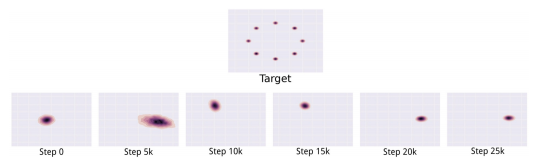
\includegraphics[width=9in]{../images/Unstable1}}

\slide{Another Example}

$${\color{red} \min_x \; \max_y xy}$$

\vfill
A Nash equilibrium is $x= y = 0$.

\vfill
Simultaneous gradient flow yields a circle.

\slide{Mode Collapse a.k.a Mode Dropping}

The generator distribution drops portions of the population.

\centerline{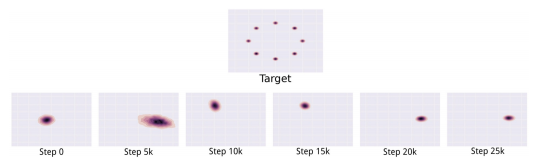
\includegraphics[width=9in]{../images/Unstable1}}

\slide{Measuring Performance}

Most evaluation of GANs is based on subjective judgments of naturalness.

\vfill
This is in contrast to language modeling where performance is directly measured by cross-entropy (bits per character or perplexity).

\slide{Summary}

GANs have not generally proved useful in discriminative tasks such as image segmentation, speech recognition, or machine translation.

\vfill
I predict that there will ultimately be better ways to model distributions (as in language modeling).

\vfill
I predict that in a few years discriminators will be limited to enforcing perceptual naturalness in applications such as
text to speech and image decompression.

\slide{END}

}
\end{document}
